% RESULTADOS-------------------------------------------------------------------

\chapter{ANÁLISE E DISCUSSÃO DOS RESULTADOS}
\label{chap:analise-resultados}

Devido à complexidade dos circuitos, as placas desta etapa do projeto não foram produzidas como protótipos artesanais, como foi feito com as PCIs da Matriz durante o Programa de Iniciação Científica. As placas aqui projetadas possuem uma grande quantidade de vias (furos metalizados que interligam as faces), trilhas e isolação (separação mínima entre as trilhas) muito pequenas, o que tornaria inviável sua fabricação no Laboratório de Corrosão por falta de material adequado. Portanto, os projetos dessas PCIs foram enviados diretamente para a fabricação industrial.

A \autoref{fig:pci-interface} apresenta a placa de circuito impresso da Interface, já com seus componentes montados. Foi fabricada por uma empresa da região de Nova Trento, em Santa Catarina, a de orçamento mais acessível entre as quase 20 empresas contatadas. Trata-se de uma produção industrial, inclusive com a garantia de integridade por meio de testes elétricos.

\begin{figure}[H]
    \centering
    \caption{Placa de circuito impresso da Interface}
    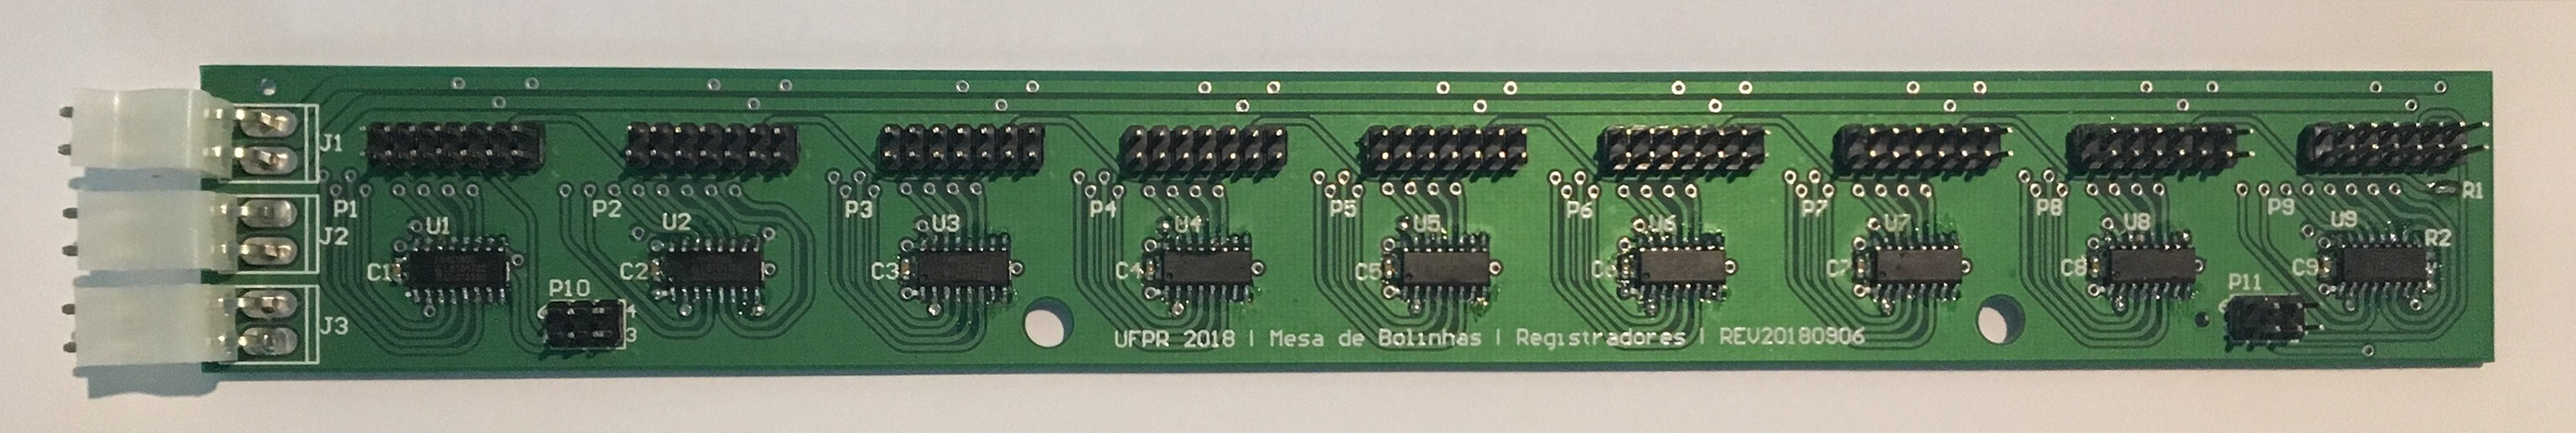
\includegraphics[width=0.99\textwidth]{./dados/figuras/pci-interface}
    \fonte{(O AUTOR, 2018)}
    \label{fig:pci-interface}
\end{figure}

Com relação à placa de circuito impresso da seção de controle, após contatar mais de 20 empresas, somente cerca de 3 delas teriam capacidade de produzir PCIs com tamanhas dimensões (500 mm x 90 mm), sendo que os valores ultrapassavam os R\$1000,00. Então, decidiu-se reprojetar a placa do Controlador, na verdade, separá-la em outras 3 PCIs, como apresentado na \autoref{fig:controlador-corte}. Dessa forma, as PCIs teriam as dimensões adequadas para produção na maioria das empresas. Ademais, as placas seriam conectadas por meio de resistores de $0\Omega$ (encapsulamento SMD 1206), dispensando o uso de fios. 

\begin{figure}[H]
    \centering
    \caption{Reprojeto da placa de controle, detalhe para os locais de corte e resistores de conexão}
    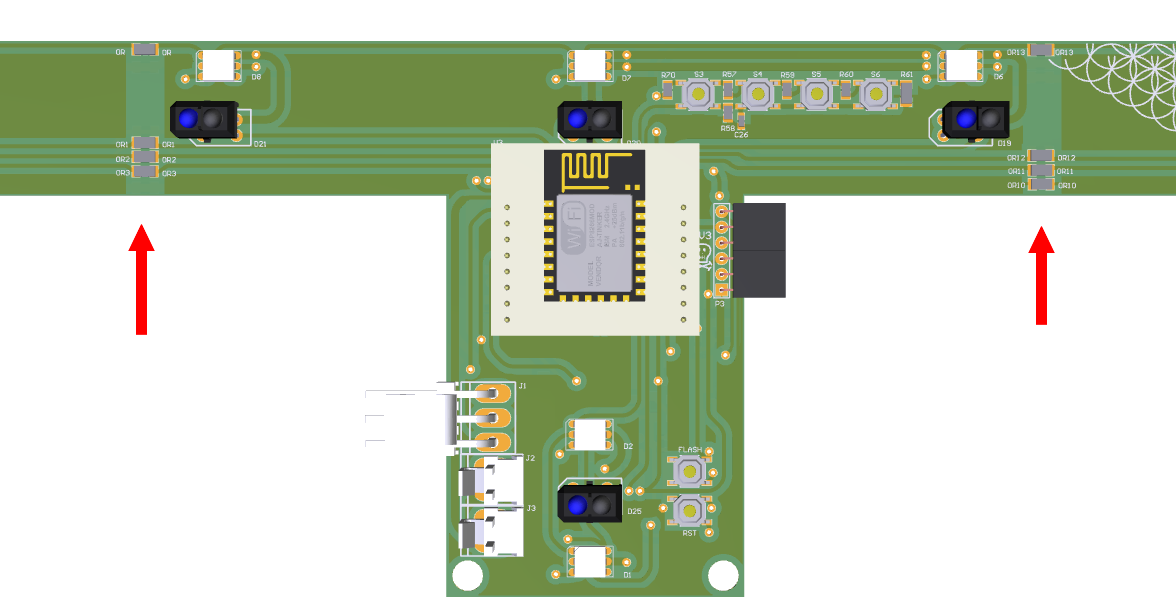
\includegraphics[width=0.7\textwidth]{./dados/figuras/controlador-corte}
    \fonte{(O AUTOR, 2018)}
    \label{fig:controlador-corte}
\end{figure}

Contudo, como mencionado no \autoref{chap:metodologia}, cada modelo de placa é considerado um projeto íntegro pelas fabricantes de PCIs e, em virtude do pedido mínimo, o valor total ainda seria alto. Então, as placas foram enviadas para a fabricação em uma universidade da região de Curitiba, que conta com um laboratório de produção de protótipos, inclusive com confecção de vias metalizadas. As Figuras \ref{fig:controlador-esq}, \ref{fig:controlador-dir} e \ref{fig:controlador-cen} apresentam os protótipos fabricados.

\begin{figure}[H]
    \centering
    \caption{Placa Esquerda do Controlador}
    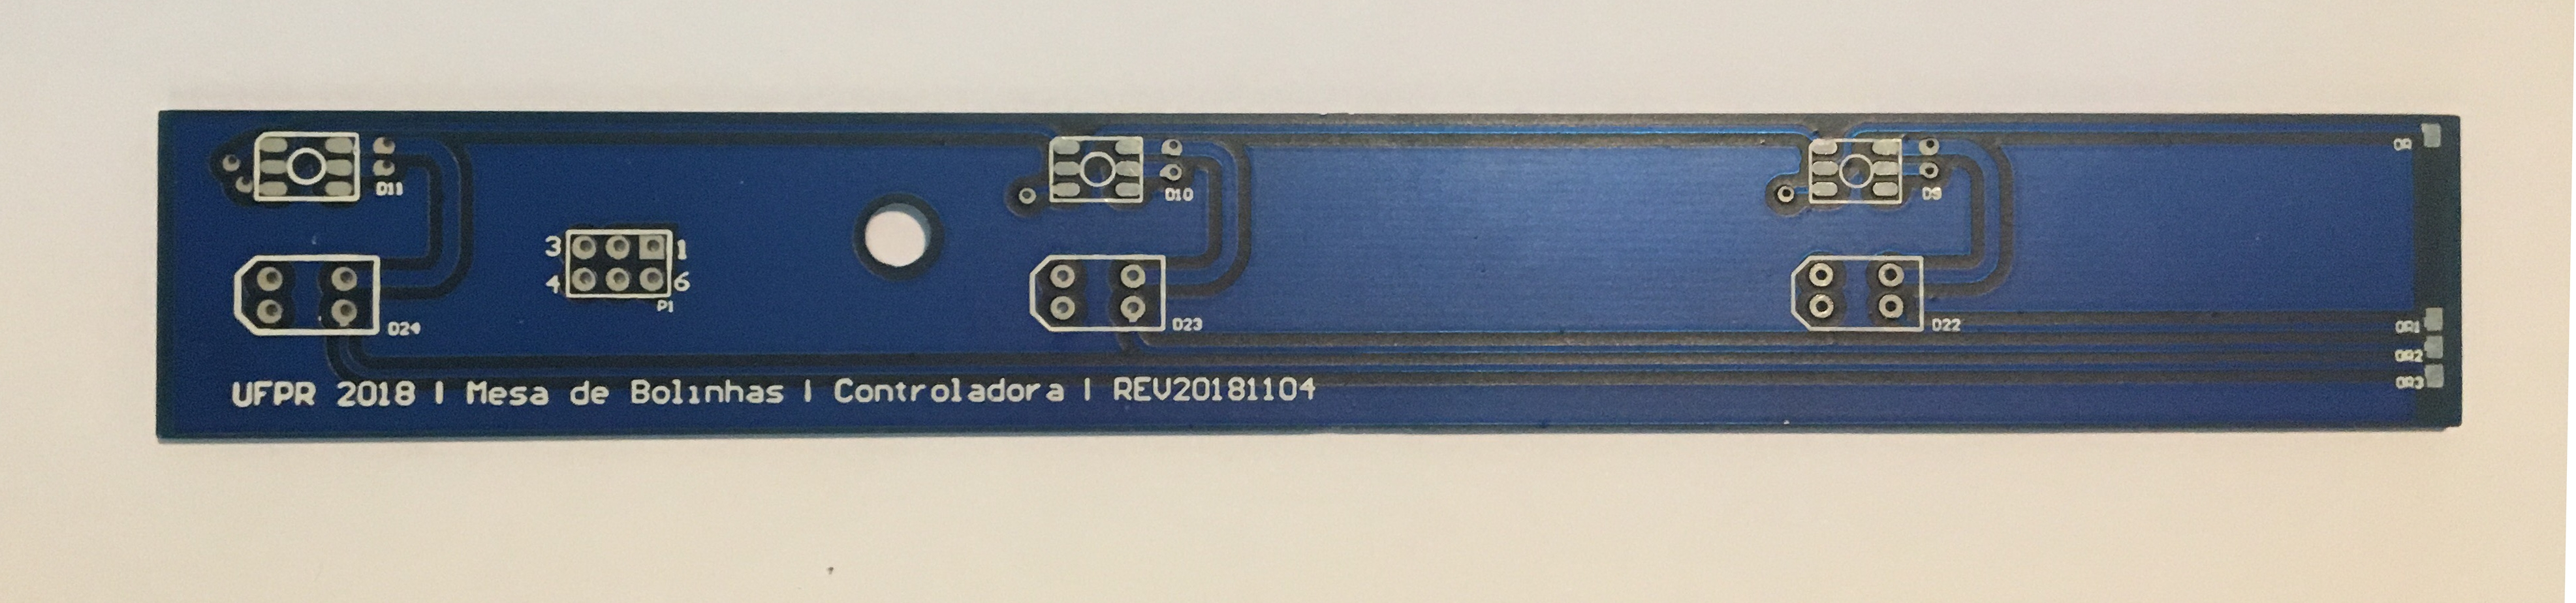
\includegraphics[width=0.9\textwidth]{./dados/figuras/controlador-esq}
    \fonte{(O AUTOR, 2018)}
    \label{fig:controlador-esq}
\end{figure}

\begin{figure}[H]
    \centering
    \caption{Placa Direita do Controlador}
    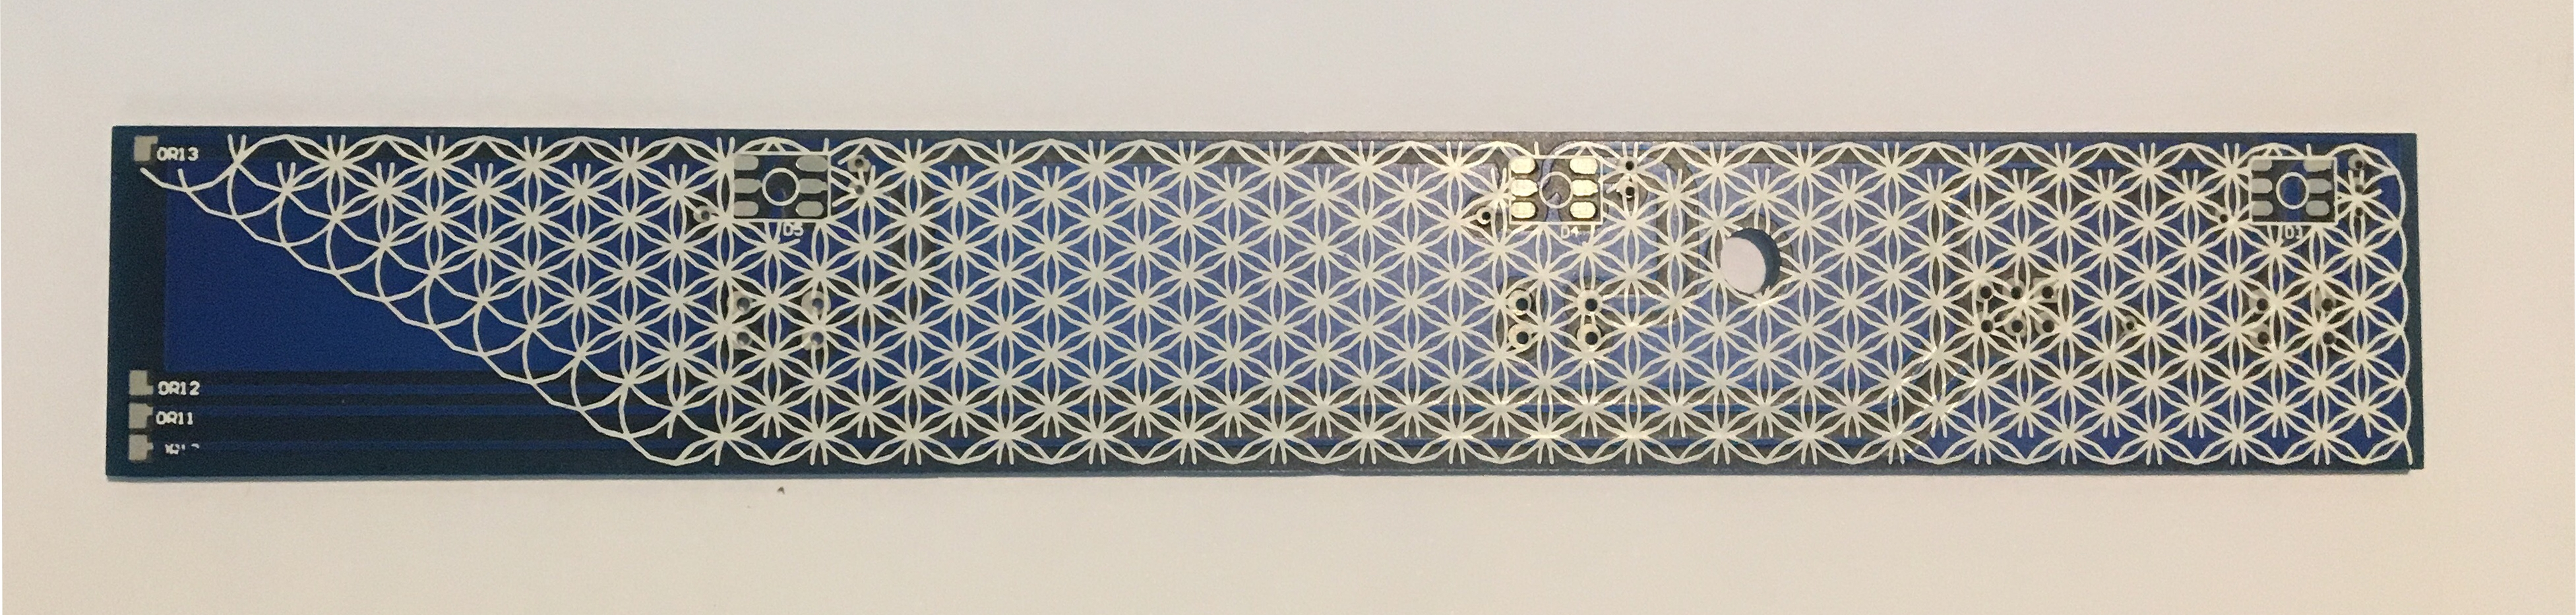
\includegraphics[width=0.9\textwidth]{./dados/figuras/controlador-dir}
    \fonte{(O AUTOR, 2018)}
    \label{fig:controlador-dir}
\end{figure}

\begin{figure}[H]
    \centering
    \caption{Placa Central do Controlador, parcialmente montada}
    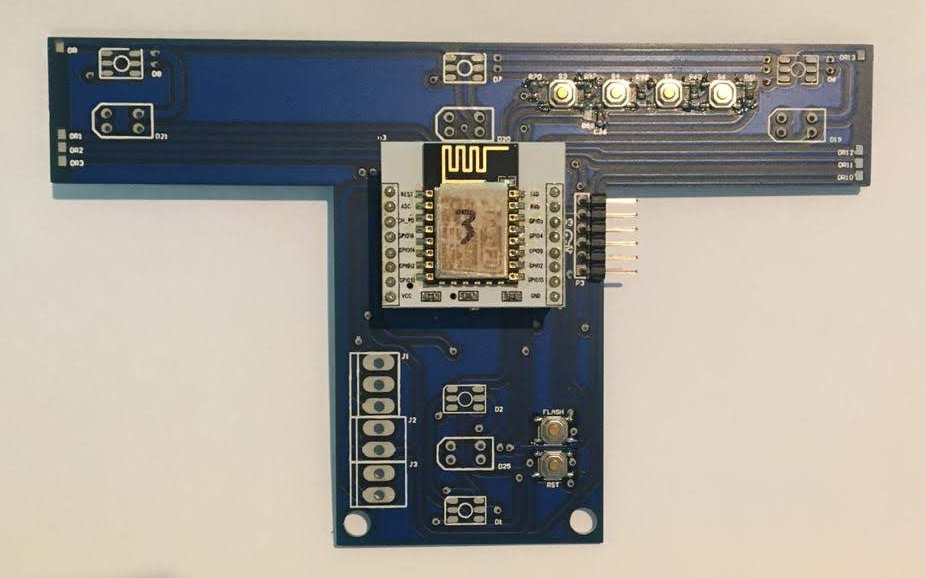
\includegraphics[width=0.8\textwidth]{./dados/figuras/controlador-cen}
    \fonte{(O AUTOR, 2018)}
    \label{fig:controlador-cen}
\end{figure}

Visto a carência de várias técnicas de roteamento do \emph{software} de leiaute utilizado durante o Programa de Iniciação Científica, o autor optou por usar um \emph{software} mais avançado para o desenvolvimento deste projeto (Interface e Controlador). Entretanto, devido à inexperiência com o novo programa e também à sua complexidade, maior que a do \emph{software} anterior, o andamento do projeto já vinha atrasado em relação ao cronograma. Além disso, houve dificuldade na montagem das placas do Controlador. Por se tratarem de protótipos produzidos de maneira semi-industrial, o acabamento da superfície exposta (terminais de cobre) é de qualidade muito inferior ao das placas fabricadas de forma industrial (PCIs da Interface). A \autoref{fig:comparacao-pads} \footnote{A imagem está distorcida devido à lente de aproximação.} apresenta a comparação dos dois modelos: à esquerda, o protótipo do Controlador, e à direita, a placa da Interface, produzida de forma industrial. Nota-se que o acabamento da placa do Controlador é mais fosco que o da Interface, mais granuloso. Esse material é de difícil aderência ao estanho através do ferro de solda. Talvez, o mais indicado seria a montagem por meio de uma estação de solda por ar quente, que alcança de maneira uniforme toda a área a ser soldada, além do fluxo especial da pasta de solda. Entretanto, nem o autor, nem a universidade dispõem desse equipamento.

\begin{figure}[H]
    \centering
    \caption{Comparação do acabamento dos terminais de solda}
    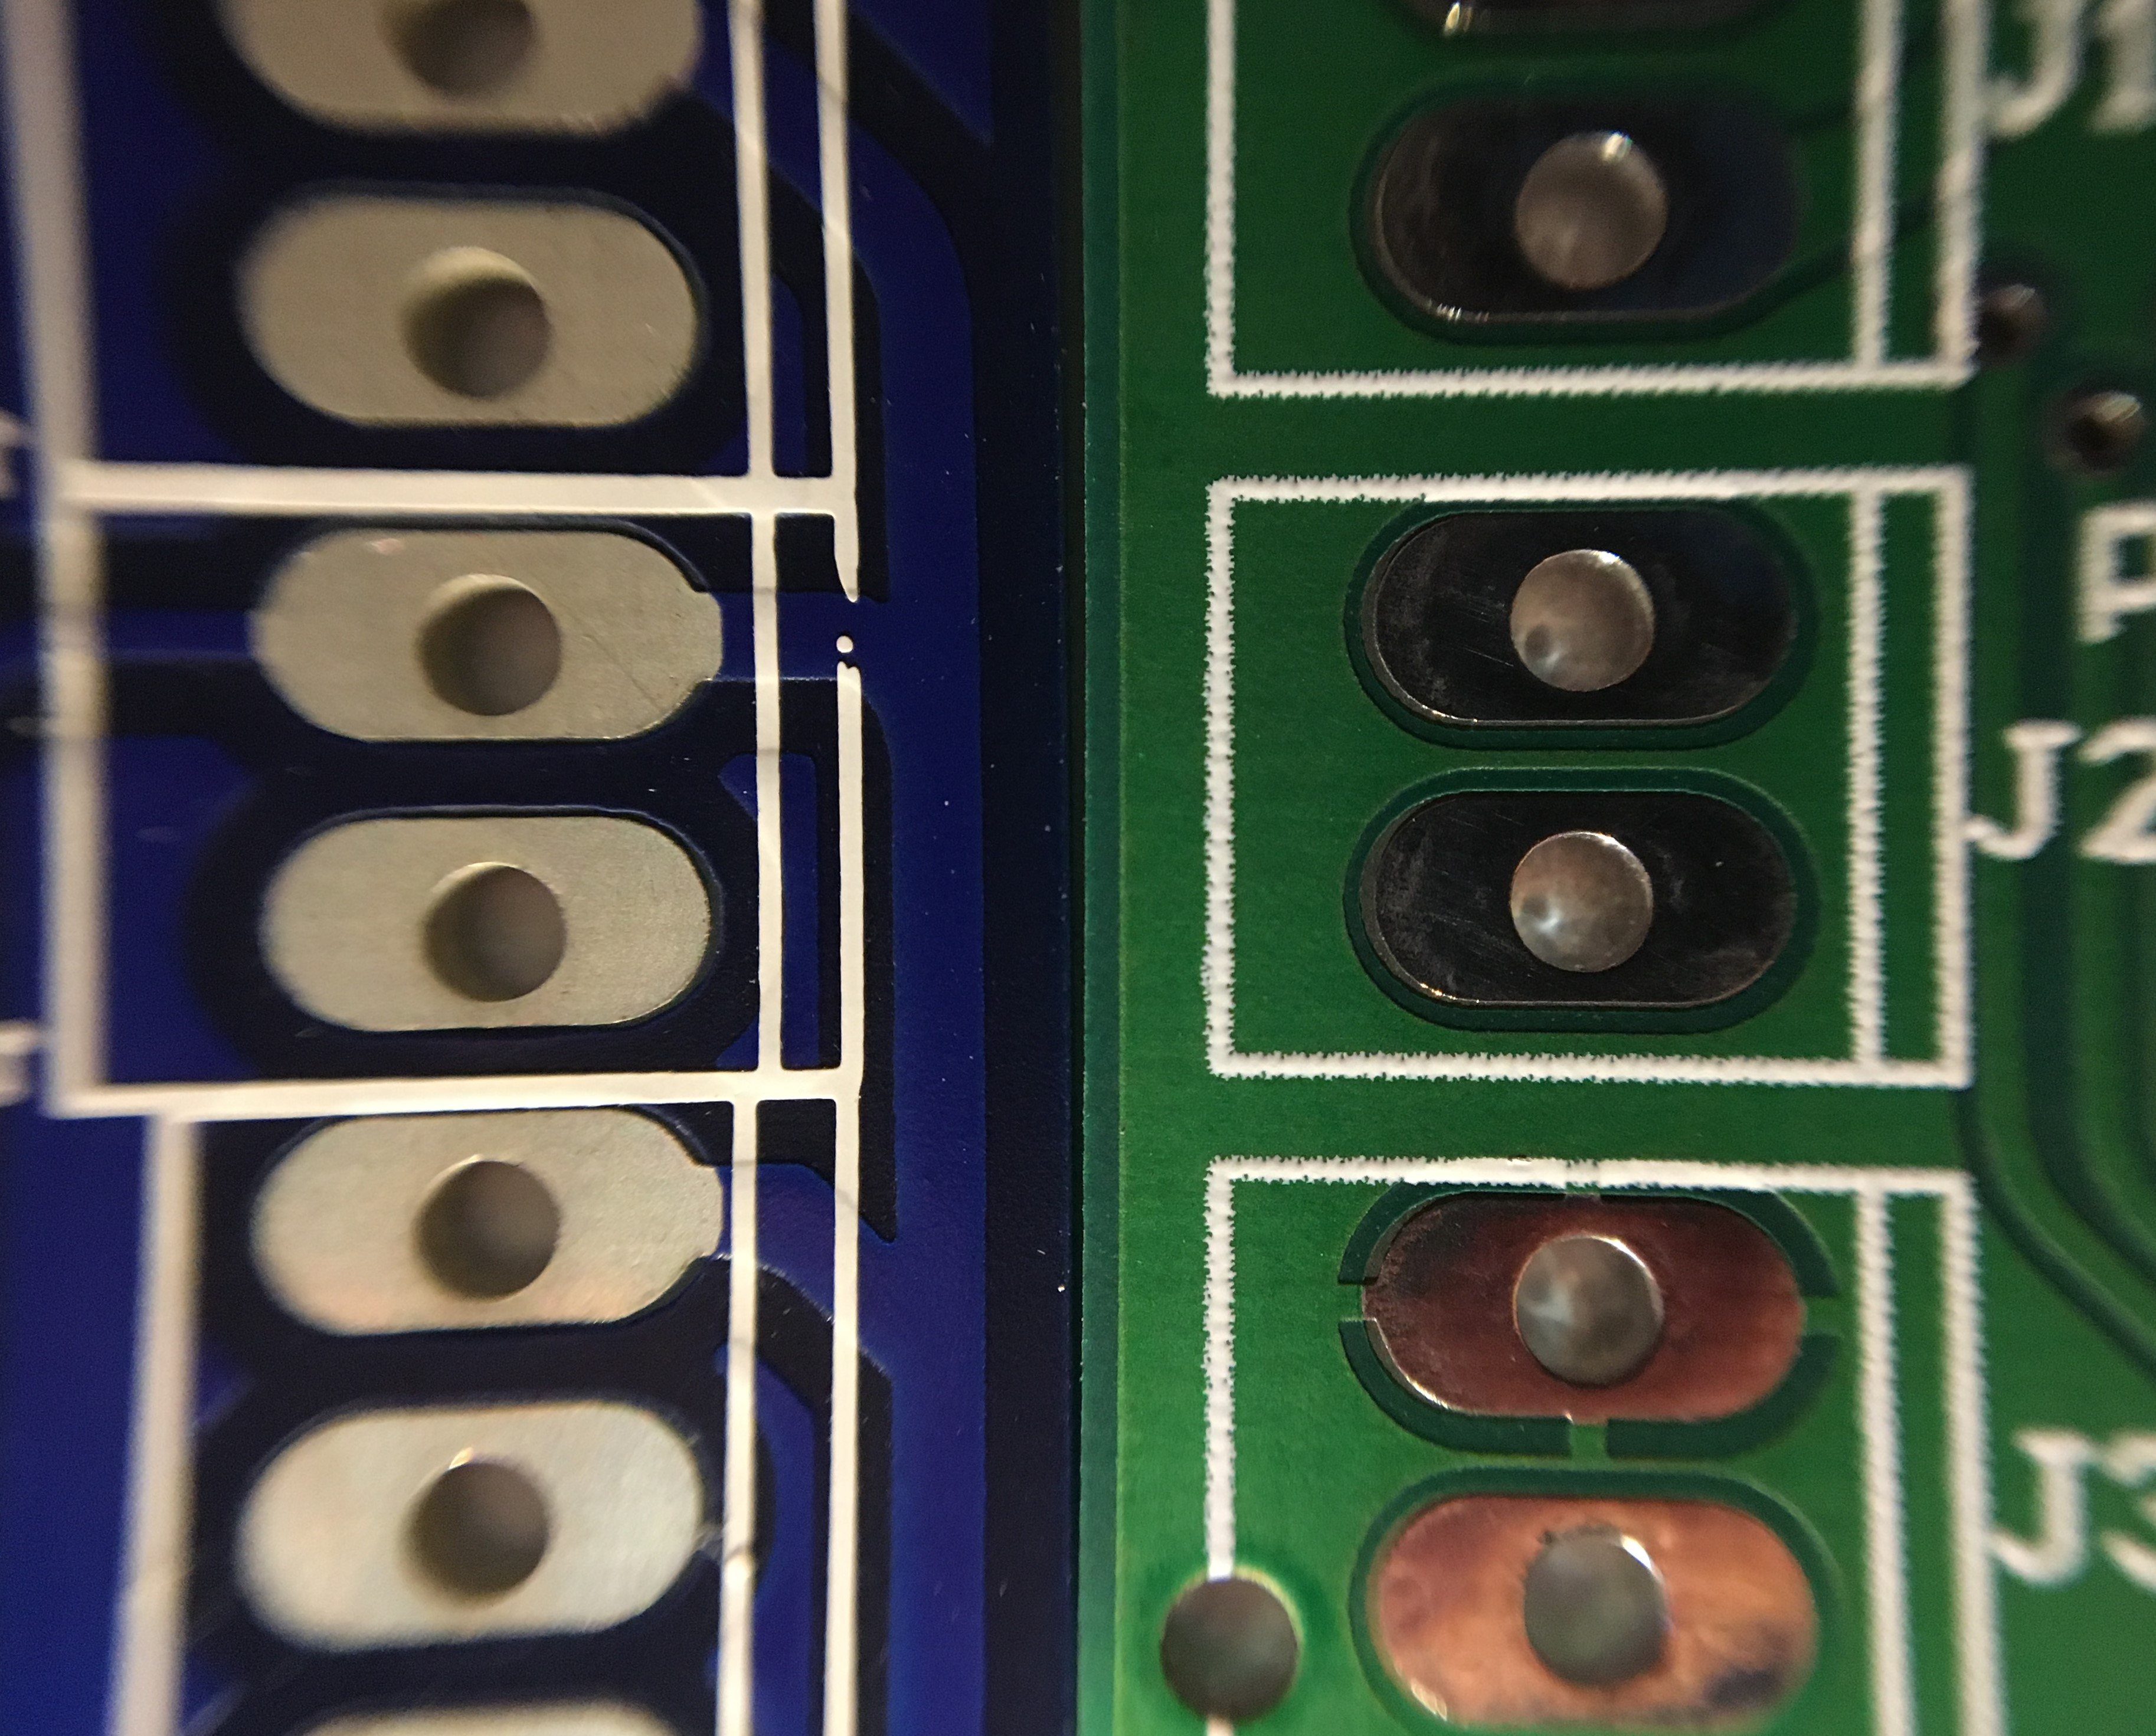
\includegraphics[width=0.7\textwidth]{./dados/figuras/comparacao-pads}
    \fonte{(O AUTOR, 2018)}
    \label{fig:comparacao-pads}
\end{figure}

Em função da placa de controle não ter sido finalizada dentro do período do cronograma, não foi possível testar o \emph{firmware} desenvolvido, que já estava em uma etapa avançada, porém ainda não havia sido testado, uma vez que dependia dos periféricos do Controlador. O código das implementações se encontram na seção de Apêndices, sendo: inicialização dos periféricos internos, inicialização dos periféricos externos, técnica de \emph{debounce} e fila de eventos. Faltando apenas a máquina de estados finita dos LEDs.
